
\section{Linux}
If using another operating system create a virtual machine with Ubuntu. If you are already using Linux then you should not need to do anything. Much of what we do will be based on Ubuntu 18.04 LTS (64 bit).

Create a directory CST4025 and a subdirectory 1. Save all your work in this directory. 


\section{Cryptographic Hash}
MD5 \cite{rivest:md5} is possibly the most popular hashing algorithm, this does not mean it is the best. For a review of hashing algorithms see \cite{rogaway:shrimpton, yaga2018blockchain}. In this exercise we are going to use Secure Hash Algorithm (SHA, \cite{sha1}) with 256-bit mode output.  

Create 8 files as shown in Table \ref{ta:ex1}, you can do this manually or write a program.

\begin{table}[tbh!]
	\centering
	\begin{tabular}{l|r}\hline
		{\bf Filename}	&	{\bf Content} \\ \hline \hline
		0.txt		&	0 \\
		1.txt		&	1 \\ 
		2.txt		&	2 \\ 
		3.txt		&	3 \\
		4.txt		&	4 \\
		5.txt		& 	5 \\
		6.txt		&	6 \\
		7.txt		&	7 \\ \hline
		%8.txt		&	8 \\
		%9.txt		&	9 \\
	\end{tabular}
	\caption{ Eight Files with a single digit}
	\label{ta:ex1}
\end{table}

Let's complete a hash for the first file, `0.txt', type the following: \\
{\tt shasum -a 256 0.txt}

The `{\tt shasum}' is the command. The '{\tt a}' switch is followed by the value of 256, which is the algorithm selected. Finally, the filename is provided. The output should be as follows:\\
{\tt\scriptsize 5feceb66ffc86f38d952786c6d696c79c2dbc239dd4e91b46729d73a27fb57e9  0.txt}\\
\normalsize

You should have 8 files, find the cryptographic hash for SHA using 256 output? The output to all the files is shown below:\\
{\tt\scriptsize
5feceb66ffc86f38d952786c6d696c79c2dbc239dd4e91b46729d73a27fb57e9  0.txt\\
6b86b273ff34fce19d6b804eff5a3f5747ada4eaa22f1d49c01e52ddb7875b4b  1.txt\\
d4735e3a265e16eee03f59718b9b5d03019c07d8b6c51f90da3a666eec13ab35  2.txt\\
4e07408562bedb8b60ce05c1decfe3ad16b72230967de01f640b7e4729b49fce  3.txt\\
4b227777d4dd1fc61c6f884f48641d02b4d121d3fd328cb08b5531fcacdabf8a  4.txt\\
ef2d127de37b942baad06145e54b0c619a1f22327b2ebbcfbec78f5564afe39d  5.txt\\
e7f6c011776e8db7cd330b54174fd76f7d0216b612387a5ffcfb81e6f0919683  6.txt\\
7902699be42c8a8e46fbbb4501726517e86b22c56a189f7625a6da49081b2451  7.txt\\
}

\section{Merkle Tree}
Merkle Trees are binary hash tree. With files `0.txt' and `1.txt' build a single hash tree as shown in Fig. \ref{fi:hashtree1}
\begin{itemize}
	\item shasum -a 256 *.txt $>$ files.sha
\end{itemize}

\pagebreak
\begin{figure}[h!]
	\centering
	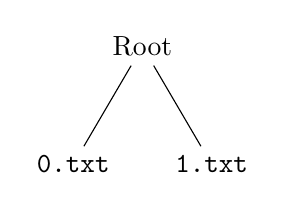
\begin{tikzpicture}[sibling distance=5em]
		\node{Root}
			child{ node {\tt 0.txt}}
			child{ node {\tt 1.txt}};
	\end{tikzpicture}
	\caption[Caption for LOF]{Simple binary hash tree: Concatenate hashes from `0.txt' and `1.txt': 5feceb66ffc86f38d952786c6d696c79c2dbc239dd4e91b46729d73a27fb57e9 6b86b273ff34fce19d6b804eff5a3f5747ada4eaa22f1d49c01e52ddb7875b4b. Hash this to get the root: \\cf1ba4395883ffc50f87999888e810feb5deb92498f3c9cd48a4ef7e063a3b37 \protect\footnotemark}
\label{fi:hashtree1}
\end{figure}
\footnotetext{This is the result of converting the hexidecimal to a string and inserting new lines between each hash.}
	
Calculate the merkle root for all eight files?
If you allow for linebreaks between each hash, the answer for the root should be:\\ 
9182e69210a41e2592ae15f11bb237bd45642f173e285e311c4054282b04e0d7


\section{Cryptographic Hash Functions}
Hashing is an important component to the blockchain, slight variations in the file cause a huge variation in the resulting hash. Often hashes are represented mathematically, as shown in Eq. \ref{eq:hash}
\begin{equation}\label{eq:hash}
	H_{a}(x) = d
\end{equation}

where $H$ is the hash function, $a$ is the hashing algorithm used (in our case SHA256), $x$ is the message and $d$ is the digest. How would it be possible for Eq. \ref{eq:hash2} to be correct.

\begin{equation}\label{eq:hash2}
	H_{a}(x) = H_{a}(y)
\end{equation}

\pagebreak
\subsection{Properties}
Important properties of cryptographic hash functions are:
\begin{enumerate}
	\item {\bf Pre-image resistant}
	\item {\bf Second pre-image resistant}
	\item {\bf Collision resistant}
\end{enumerate}

Write definitions for each of these properties above?
	
\subsection{Nonces}
Nonces play an important part in blockchain consensus algorithms, in particular the proof of work (PoW) consensus algorithm used in Bitcoin. The nonce is added to the data and is a way of changing the digest without changing the data. Eq. \ref{eq:nonce} shows how nonces are used:
\begin{equation}\label{eq:nonce}
	H_{a}(concat(x,n))=d
\end{equation}


where $H$ is the hash function, $a$ is the hashing algorithm used, $d$ is the digest, $x$ is the original data message, and $n$ is the nonce. The function 'concat(x,n)', concatenates the two strings. By changing the value of the nonce the digest can change, without altering the data.

The next exercise is to test Proof-of-work consensus algorithm. The nonce is 4 characters in length and is added to the original message. The target is a hex value less than the digest, so $H_{a}(x+n)<H_{a}(x)$. Anything less than this is accepted. Write a program to complete this?

%see nonce.py

%\section{Blockheads}
%
%Download blockhead.tar from myLearning. This is a simple blockchain, consisting of 3 blocks and the abstract structure is displayed in Fig. \ref{fi:blockhead}
%
%
%\begin{figure}
%	\centering
%	\begin{tikzpicture}
%			
%		\node [bank] 	at (0,4) (1){Prev. Hash};
%		\node [bank] 	at (0,0) (2){Merkle Root};
%		\node [bank]	at (4,4) (3){Timestamp};
%		\node [bank]    at (4,0) (4){Signature};
%
%	\end{tikzpicture}
%	\caption{Abstract of each block in blockheads}
%	\label{fi:blockhead}
%\end{figure}
%
%Change the genesis block in the blockchain, and record the steps you have to take?
%


